\part{Wikipedia-based Explicit Semantic Analysis}
\label{part:ESA}
\chapter[ESA]{Wikipedia-based Explicit Semantic Analysis}
\initial{N}{atural} language processing has long been both a subject of interest and a source of great challenges in the field of artificial intelligence\todo{ref}. The difficulty varies greatly depending with the different language processing tasks; certain problems, such as text categorization, are relatively straightforward to convert to a purely mathematical problem, which in turn can be solved by a computer, whereas other problems, such as computing semantic relatedness, necessitates a deeper understanding of a given text, and thus poses a greater problem. This sections aims firstly to give a brief introduction to some of the most prominent techniques used in language processing in order to explain my chosen method of explicit semantic analysis (ESA), and secondly to explain in detail my practical implementation of an ESA-based text interpretation scheme.

\section{Methods}
This section outlines a few methods used in natural language processing, going into some detail on ESA while touching briefly upon related techniques.

\subsection{Bag-of-Words}
An example of a categorization problem is the 'bag of words' approach, which has seen use in spam filters.\todo{ref} Here, text fragments are treated as unordered collections of words drawn from various bags, which in the case of spam filters would be undesired mails (spam) and desired mails (ham). By analysing large amounts of regular mail and spam, the probability of drawing each of the words constituting a given text from each bag can be computed, and the probability of the given text fragment representing draws from each bag can be computed using Bayesian statistics.

More formally, the text $T$ is represented as a collection of words $T = \cb{w_1, w_2, \ldots, w_n}$, and the probability of  $T$ actually representing draws from bag $j$ is hence
\begin{align}
\begin{split}
		P(B_j|T) &= \dfrac{P(T|B_j)P(B_j)}{P(T)}, \\
		&= \dfrac{\prod_i P(w_i|B_j)P(B_j)}{\sum_j\prod_i P(w_i|B_j)P(B_j)}, \label{eqn:bayesian_bow_thingy}
\end{split}
\end{align}
for an arbitrary number of bags labelled by $j$. This method is simple and powerful whenever a text is expected to fall in one of several discrete categories (such as spam filters or language detection\todo{ref}). However, for more complex tasks it proves lucrative to attempt instead to assign some kind of meaning to text fragments rather than to consider them analogous to lottery numbers or marbles. As an intuitive example of the insufficiency of the bag-of-words approach in more complex tasks, consider the problem of determining how related one text fragment is to another, which I'll treat in detail in section \ref{sec:social_media_impact} in order to determine the degree in which a media campaign has impacted a series of texts mined from social media. A simplified example of a media campaign by Google for their augmented reality product 'Google Glass' could be the text fragment 'Google unveils Google Glass'. If, in reaction to this, an excited user writes 'Larry Page launches intelligent eyewear', a naive bag-of-words like \eqref{eqn:bayesian_bow_thingy} would determine that the words in the user's exclamation could not have been drawn from the 'bag' represented by Google's campaign and so would wrongfully conclude that the two are unrelated. A more reasonable approach would assign some meaning to the words in which 'Larry Page' (Google's CEO) and 'Google', and 'Google Glass' and 'intelligent eyewear' are highly related, just as 'unveil' and 'launch' should be ascribed similar meanings.

This notion of meaning will be elaborated on shortly, as it varies depending on the method of choice, but the overall idea is to ascribe to words a meaning which depends not only on the word itself, but also on the connection between the word and and existing repository of knowledge. The reader may think of this as mimicking the reading comprehension of humans. In itself, the word 'dog' for instance, contains a mere 24 bits of information if stored with a standard encoding, yet a human reader immediately associates a rich amount of existing knowledge to the word, such as dogs being mammals, related to wolves, being a common household pet, etc. The objective of both explicit and latent semantic analysis is to establish a high-dimensional 'concept space' in which words and text fragments are represented as vectors. The difference between explicit and latent semantic analysis is the method used to obtain said concepts, a explained in the following sections.

\subsection{Semantic Analysis}
\label{sec:semantic_analysis}
Salton et al proposed in their 1975 paper \textit{A Vector Space Model for Automatic Indexing}\cite{Salton1975} an approach where words and text fragments are mapped with a linear transformation to vectors in a high-dimensional concept space,
\begin{equation}
	T \rightarrow \ket{V} = \sum_i v_i \ket{i}, v_i\in\mathbb{R}, \label{eqn:text2space}
\end{equation}
where a similarity measure of two texts can be defined as the inner product of two normalized such vectors,
\begin{equation}
	S(V,W) = \bracket{\hat{V}}{\hat{W}} = \frac{\sum_i v_i w_i}{\pp{\sum_i v_i^2}\pp{\sum_iw_i^2}}, \label{eqn:cosine_similarity}
\end{equation}
and the cosine quasi-distance can be considered as a measure of semantic distance between texts:
\begin{equation}
	D(V,W) = 1-S(V,W).
\end{equation}
This approach has later seen use in the methods of Latent Semantic Analysis (LSA) and Explicit Semantic Analysis (ESA). Both methods can be said to mimic human cognition in the sense that the transformation from \eqref{eqn:text2space} is viewed as a mapping of a text fragment to a predefined \textit{concept space} and thus, processing of texts relies heavily on external repositories of knowledge.

The difference between LSA and ESA is how the concept space is established. Although I have used solely ESA for this project, I will give an extremely brief overview of LSA for completeness following (Landauer 1998 \cite{Landauer1998}). LSA constructs its concept space by first extracting every unique word encountered in a large collection of text corpora and essentially uses the leading eigenvectors (i.e. corresponding to the largest eigenvalues) of the word-word covariance matrix as the basis vectors of its conceptual space. This is the sense in which the concept are latent - rather than interpret text in terms of explicit concepts, such as 'healthcare', LSA would discover correlations between words such as 'doctor', 'surgery' etc. and consider that a latent concept. Owing to the tradeoff between performance and computational complexity, only about 400 such vectors are kept\cite{Nakov2000}. In psychology, LSA has been proposed as a possible model of fundamental human language acquisition as it provides computers a way of estimating e.g. word-word relatedness (a task which LSA does decently) using nothing but patterns discovered in the language it encounters\cite{Landauer1998}.

In contrast, the concepts in ESA correspond directly to certain parts of the external text corpora one has employed to construct a semantic analyser. Concretely, the matrix playing the role of the reduced covariance matrix in LSA has columns corresponding to each text corpus used and rows corresponding to individual terms or words, with the value of each matrix element denoting some measure of relatedness between the designated word and concept. I have used the English Wikipedia, so naturally each concept consists of an article, although the process could easily be tuned to be more or less fine-grained and associate instead each concept with e.g. a subsection or a category, respectively. Of course, a wholly different collection of texts could also be used - for instance a version of ESA more suited to compare the style or period of literary works could be constructed using a large collection of literature such as the Gutenberg Project. However, with no prior knowledge of the subject matter of the text to be analysed, Wikipedia seems like a good all-round solution considering its versatility and the massive numbers of volunteers constantly keeping it up to date.

I wish to point out two advantages of ESA over LSA. First, it is more successful, at least using the currently available text corpora and implementation techniques. A standard way of evaluating the performance of a natural language processing program is to measure the correlation between relatedness scores assigned to pairs of words or text fragments by the computer and by human judges. In both disciplines, ESA has outperformed LSA since it was first implemented \citat{ESA}{p 457}.

Second, the concepts employed in ESA are directly understandable by a human reader, whereas the concepts in LSA correspond to the leading moments of the covariance matrix. For example, to test whether the first semantic analyser built by my program behaved reasonably, I fed it a snippet of a news article on CNN with the headline "\textit{In Jerusalem, the 'auto intifada' is far from an uprising}". This returned an ordered list of top scoring concepts as follows:
"Hamas, Second Intifada, Palestinian National Authority, Shuafat, Gaza War (2008-09), Jerusalem, Gaza Strip, Arab Peace Initiative, Yasser Arafat, Israel, West Bank, Temple Mount, Western Wall, Mahmoud Abbas", which seems a very reasonable output.

\section{Constructing a Semantic Analyser}
The process of applying ESA to a certain problem may be considered as the two separate subtasks of first a very computationally intensive construction af the machinery required to perform ESA, followed by the application of said machinery to some collection of texts. For clarity, I'll limit the present section to the details of the former subtask while description its application and results in section \ref{sec:esa_results}.

The construction itself is divided into three steps which are run in succession to create the desired machinery. The following is a very brief overview of these steps, each of which is elaborated upon in the following subsections.
\begin{enumerate}
	\item First, a full Wikipedia XML-dump%
	\footnote{These are periodically released at \url{http://dumps.wikimedia.org/enwiki/}}
	is parsed to a collection of files each of which contains the relevant information on a number of articles. This includes the article contents in plaintext along with some metadata such as designated categories, inter-article link data etc.
	\item Then, the information on each concept (article) is evaluated according to some predefined criteria, and concepts thus deemed inferior are purged from the files. Furthermore, two list are generated and saved, which map unique concepts and words, respectively, to an integer, the combination of which is to designate the relevant row and column in the final matrix. For example, the concept 'Horse' corresponded to column $699221$ in my matrix, while the word 'horse' corresponded to row $11533476$.
	\item Finally, a large sparse matrix containing relevance scores for each word-concept pair is built and, optionally, pruned (a process used to remove 'background noise' from common words as explained in section \ref{sec:matrix_building})
\end{enumerate}
These steps are elaborated upon in the following.

\subsection{XML Parsing}
The Wikipedia dump comes in a rather large ($\sim$50GB unpacked for the version I used) XML file which must be parsed to extract each article's contents and relevant information. This file is essentially a very long list of nested fields where the data type in each field is denoted by an XML tag, such as \verb+<text> blabla </text>+. A very simplified example of a field for one Wikipedia article is shown in \ref{code:xml_example}
%
\floatcode[language = XML, caption={A simplified snippet, of a Wikipedia XML dump.}, label = code:xml_example]{pics/wiki_example.xml}
%\lstinputlisting[float=ht, style=snippet, language=XML, caption = A simplified snippet of a Wikipedia XML dump., label = code:xml_example]{pics/wiki_example.xml}
%
The content of each field has already been sanitised by Wikipedia so that if for instance the symbol '$<$' is entered into an article, it is instead represented as '\&lt' in the XML file.
To this end, I wrote a SAX parser, which processes the dump sequentially to accommodate its large size. When running, the parser walks through the file and sends the various elements it encounters to a suitable processing function depending on the currently open XML tag. For example, when a 'title' tag is encountered, a callback method is triggered which assigns a column number to the article title and adds it to the list of processed articles. For the callback method for processing the 'text' fields, I used a bit of code from the pre-existing Wikiextractor project to remove Wiki markup language (such as links to other articles being displayed with square brackets and the like) from the content. This code is included in section \ref{sec:wikicleaner.py}. The remainder of the parser is my work, and is included in section \ref{sec:xml_parse.py}. Throughout this process, the parser keeps a list of unique words encountered as well as outgoing link information for each article. These lists, along with the article contents, are saved to files each time a set number of articles have been processed. The link information is also kept in a hashmap with target articles as keys and a set articles linking to the target as values. The point of this is to reduce the computational complexity of the link processing as detailed in the following section.

\subsection{Index Generation}
The next step reads in the link information previously saved and adds it as ingoing link information in the respective article content files. The point of this approach is that link information is initially saved as a hashmap so the link going to a given article can be found quickly, rather that having to search for outgoing links in every other article to determine the ingoing links to each article, which would be of $\bigo{n^2}$ complexity.

Following that, articles with sufficiently few words and/or in\-going/\-out\-going links are discarded an index lists for the remaining articles and words are generated to associate a unique row/column number with each word/concept pair. The code performing the step described here is included in section \ref{sec:generate_indices.py}.

\subsection{Matrix Construction}
\label{sec:matrix_building}
This final step converts the information compiled in the previous steps into a very large sparse matrix. The program allows for this to be done in 'chunks' in order to avoid insane RAM usage. Similarly, the matrix is stored in segments with each file containing a set number of rows in order to avoid loading the entire matrix to interpret a short text.

The full matrix is initially constructed using a DOK (dictionary of keys) sparse format in which the $i,j$th element simply counts the number of occurrences of word $i$ in the article corresponding to concept $j$. This is denoted $\text{count}(w_i,c_j)$. The DOK format as a hashmap using tuples $(i,j)$ as keys and the corresponding matrix elements as values and is the fastest format available for element-wise construction. The matrix is subsequently converted to CSR (compressed sparse row) format, which allows faster operations on rows which performs much quicker when computing TF-IDF (term frequency - inverse document frequency) scores and extracting concept vectors from words, i.e. when accessing separate rows corresponding to certain words.

Each non-zero entry is then converted to a TF-IDF score according to
\begin{equation}
	T_{ij} = \pp{1 + \ln{\pp{\text{count}(w_i, c_j)}}} \ln{\pp{\frac{n_c}{df_i} }}, \label{eqn:TF-IDF}
\end{equation}
where $n_c$ is the total number of concepts and
\begin{equation}
	df_i = \left| \left\{ c_k, w_i \in c_k \right\} \right|
\end{equation}
is the number of concepts whose corresponding  article  contains the  $i$th word. Thus, the first part of \eqref{eqn:TF-IDF}, $1 + \ln{\pp{\text{count}(w_i, c_j)}}$ is the \textit{text frequency} term, as it increases with the frequency of word $i$ in document $j$. Similarly, $\ln{\pp{\frac{n_c}{df_i} }}$ in \eqref{eqn:TF-IDF} is the \textit{inverse document frequency} term as it decreases with the frequency of documents containing word $i$. Thus, the TF-IDF score as somewhat complement to entropy \todo{Giver det mening?} in that it goes to zero as the fraction of documents containing word $i$ goes to 1, and takes its highest values if word $i$ occurs with high frequency in only a few documents\cite{Manning2009}. While \eqref{eqn:TF-IDF} is not the only expression to have those properties, empirically it tends to achieve superior results in information retrieval\cite{Salton1988}.

Each row is then $L^2$ normalized (divided by their Euclidean norm):
\begin{equation}
	T_{ij} \rightarrow \frac{T_{ij}}{\sqrt{\sum_i T_{ij}^2}}.
\end{equation}
Finally, each row is pruned to reduce spurious associations between concepts and articles with a somewhat uniform occurrence rate. This was done in practice by following the pragmatic approach of Gabrilovich \cite{ESA} of sorting the entries of each row, move a sliding window across the entries, truncating when the falloff drops below a set threshold and finally reversing the sorting.
\todo{Hearst nævner noget offentligt tilgængeligt Reuters-data som folk øver tekstklassifikation på. Det kunne være ret sjovt. Det kunne være sjovt at lave 'semantisk nearest neighbor'}
The result of this step is the matrix which computes the interpretation vectors as described in \ref{sec:semantic_analysis}. The code is included in section \ref{sec:matrix_builder.py}.


\section{Applications \& Results}
\label{sec:esa_results}
Having constructed a necessary machinery, I wrote a small Python module to provide an easy-to-use interface with the output from the computations described earlier. The code for this is included in section \ref{sec:cunning_linguistics.py}. The module consists mainly of a SemanticAnalyser class, which loads in the previously mentioned index lists and provides methods for various computations such as estimating the most relevant concepts for a text, determining semantic distance etc. For example, the following code will create a semantic analyser instance and use it to guess the topic of the input string:
\begin{snippet}[language=python]
	sa = SemanticAnalyser()
	sa.interpret_text("Physicist from Austria known for the theory of relativity")
\end{snippet}
This returns a sorted list of the basis concepts best matching the input string, where the first element is of course 'Albert Einstein'. The SemanticAnalyser class contains equally simple methods to interpret a target text file or keyboard input, to calculate the semantic similarity or cosine distance between texts, and to compute interpretations vectors from a text.

The same module contains a TweetHarvester class which I wrote in order to obtain a large number of tweets to test the semantic analyser on, as tweets are both numerous and timestamped, which allows investigations of the temporal evolution of tweets matching a given search term. The TweetHarvester class provides an equally simply interface - for instances, the 100 most recent tweets regarding a list of companies can be mined and printed by typing
\begin{snippet}[language=python]
	terms = ['google', 'carlsberg', 'starbucks']
	th = TweetHarvester()
	th.mine(terms, 100)
	print th.harvested_tweets
\end{snippet}
in addition to actively 'mining' for tweets matching a given query, the class can also passively 'listen' for tweets while automatically saving its held tweets to a generated date-specific filename once a set limit of held tweets is exceeded:
\begin{snippet}[language=python]
	th = TweetHarvester(tweets_pr_file = 100)
	th.listen(terms)
\end{snippet}
The downloaded tweets are stored as tweet objects which contain a built in method to convert to a JSON-serializable hashmap, an example of which is provided in \ref{code:tweet_example}.
%
\floatcode[caption = {Example of a downloaded tweet.}, label = code:tweet_example]{pics/tweet_example.json}
%
As can be seen in the example, the tweet object contains not only the tweets textual content but also a wide range of metadata such as the hashtags contained in the tweet, users mentioned, time of creation, language etc. Using this, I wrote a script that harvested tweets mentioning some selected brand names for about 5 months which resulted in a massive dataset of 370 million tweets. This section demonstrates some applications of the methods outlined earlier to this dataset.

\FloatBarrier
\subsection{Trend Discovery and Monitoring}
\label{sec:esa_monitoring}
A simple application of the methods outlined above is a purely exploratory analysis. As an example, using code included in section \ref{sec:esa_examples}, I extracted the 10 concepts most closely related to every tweet mentioning Carlsberg for each week over a period of a few months. This gave a bar chart like figure \ref{fig:carlsberg_exploratory_chart} for each of those weeks.
\begin{figure} %[htb]
	\centering
	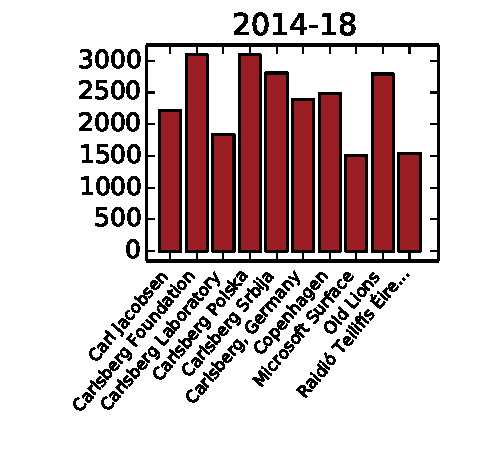
\includegraphics[width=\figwidth]{pics/esa/irish_radio_bar_chart.pdf}
	\caption{Bar chart representing the number of times various concepts appeared in the top 10 most semantically related concepts for each given tweet taken from week 18 of 2014.}
	\label{fig:carlsberg_exploratory_chart}
\end{figure}
Figure \ref{fig:carlsberg_exploratory_chart} implies some significant relation between Carlsberg and Raidió Teilifís Éireann (RTE), the Irish national radio and television service. I then discovered that RTE usually does a quarterly report on Carlsberg's earnings, and that some web sites encouraged their followers to drink Carlsberg and listen to RTE's coverage of the Eurovision Song Contest taking place in week 18 of 2014.

Another application is to manually select a few concepts of interest and then monitor how the number of tweets strongly related to them develops over time. For example I did an exploratory analysis as described above and occasionally saw the concept 'Kim Little' surface. This turned out to be a young football player signed to a team sponsored by Carlsberg, and when I produced a series of bar charts like that shown in figure \ref{fig:kim_little} and combined them into an animation, the bar representing Little tended to peak around dates on which news stories featuring her or her team could be found.
\begin{figure}
	\centering
	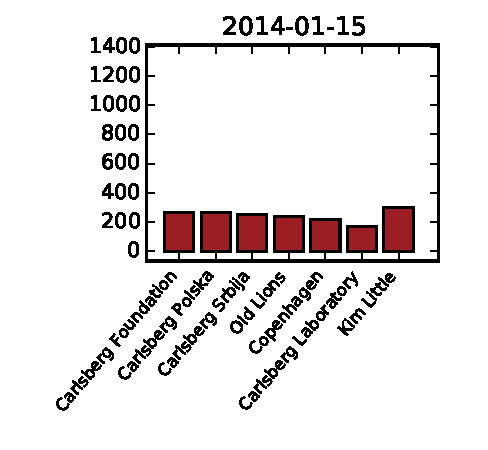
\includegraphics[width=\figwidth]{pics/esa/kim_little.pdf}
	\caption{Bar chart showing the concepts most related to tweets about Carlsberg for January 15th 2014.}
	\label{fig:kim_little}
\end{figure}
Of course these method are only effective insofar the concepts of interest actually have an associated Wikipedia article. However, these concepts are merely the basis vectors of the semantic space in which an arbitrary text can be represented, so this procedure can be extended fairly elegantly to estimate the impact of e.g. a press release on social media. This is the subject of section \ref{sec:social_media_impact}.

\FloatBarrier
\subsection{Measuring Social Media Impact}
\label{sec:social_media_impact}
One possible application of the software I wrote to perform ESA is to provide a quantitative measure of the impact of some event on social media. For instance, some corporation or organization might be interested in learning precisely effectively a campaign or press release has reached the general public as it is expressed by social media. While my tweet harvesting script was running, Google posted a blog entry%
\footnote{The original blog post is available at \url{http://googleresearch.blogspot.dk/2015/06/inceptionism-going-deeper-into-neural.html}}
on their experiments with producing psychedelic images with deep neural network called \textit{Deep Dreams} which received widespread attention on social media.

Using the text from the Deep Dreams blog post as a reference text, I converted each English tweet about Google from a period around the blog post to a semantic vector using \eqref{eqn:text2space} and computed their semantic cosine similarity with the reference text as described by \eqref{eqn:cosine_similarity}. Figure \ref{fig:deep_dreams_initial} shows this behaviour in the time around the release of the blog post.
\begin{figure} %[htb]
	\centering
	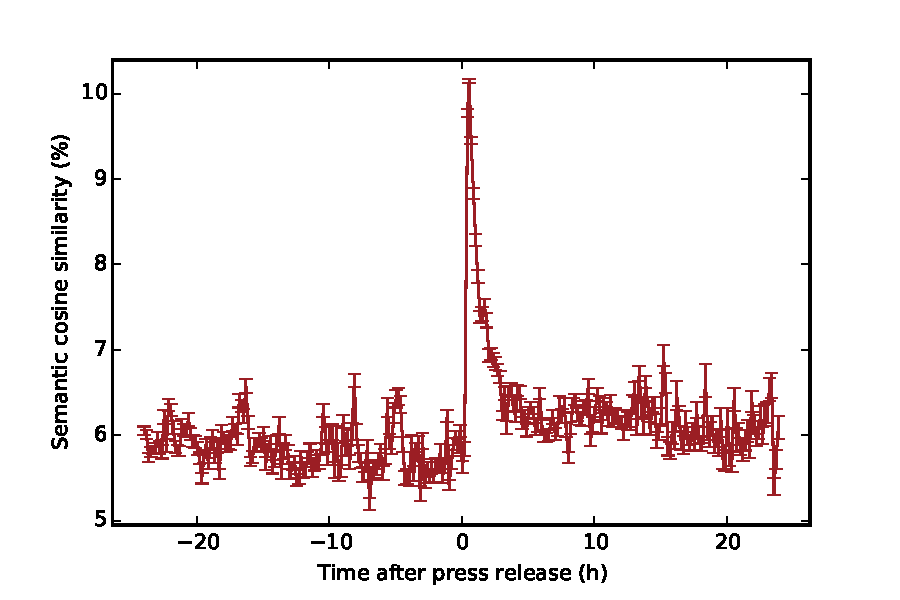
\includegraphics[width=\figwidth]{pics/esa/deep_dreams_plot_timebin.pdf}
	\caption{Graph of the mean semantic cosine similarity of tweets around the Deep Dreams press release. There is a clear peak around $t=0$ and the similarity appears increased in the period following the release. The error bars represent the true standard deviation of the sample mean $\sigma/\sqrt{N}$ for each time bin, each representing a 10-minute interval.}
	\label{fig:deep_dreams_initial}
\end{figure}
A measure of impact should of course take into account the rate at which new tweets occur. Just as one would expect, not only semantic relatedness, but also tweet frequency increase drastically around an interesting event. To make the signal from figure \ref{fig:deep_dreams_initial} independent of the normal tweet frequency, yet sensitive to changes in it, I first find the difference in semantic relatedness between the signal and a reference signal obtained long before the event to be investigated, then modulate the signal by multiplying each bin with the activity $A$ given by the ratio between the current and baseline tweet frequency. As normal Twitter activity tends to vary greatly over a 24 hour period, I obtained a baseline tweet frequency by computing the average tweet rate, weighted by the activity, for each discreet time interval of the day, and then repeating that signal into the period after the event of interest. The baseline along with the observed tweet rate is shown in figure \ref{fig:deep_dreams_counts}.
\begin{figure} %[htb]
%	\centering
	\subbottom[]{
		\begin{minipage}[t][][b]{0.45\textwidth}
			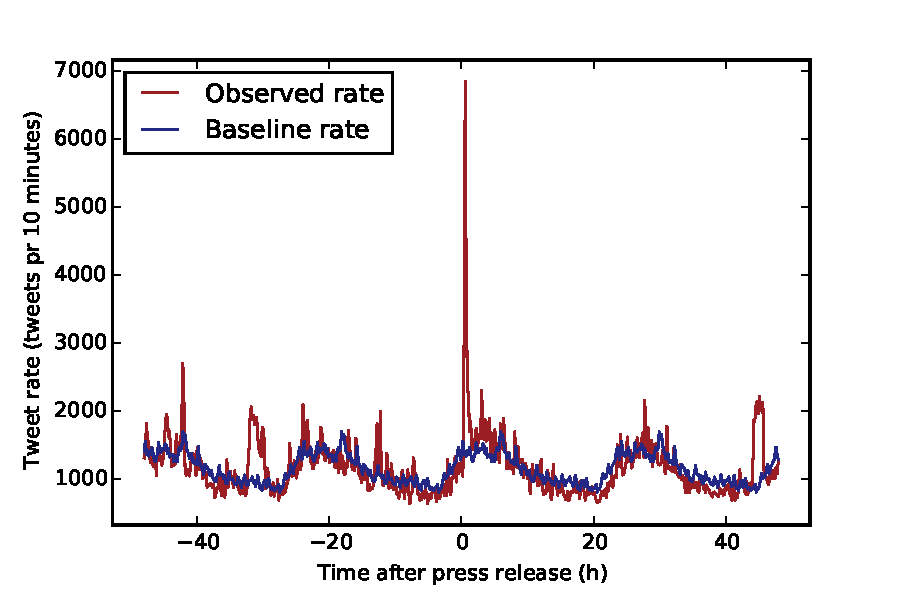
\includegraphics[width=0.5\figwidth, height=\dualheight, keepaspectratio]{pics/esa/15_07_25_counts_vs_baseline.pdf}
		\end{minipage}%
		\label{fig:deep_dreams_counts}
	}
	\subbottom[]{
		\begin{minipage}[t][][b]{0.45\textwidth}
			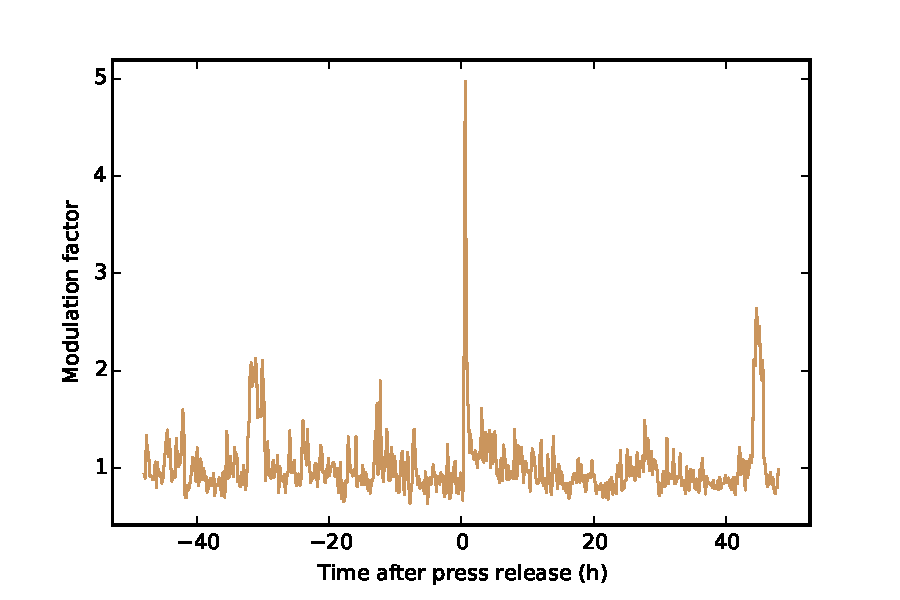
\includegraphics[width=0.5\figwidth, height=\dualheight, keepaspectratio]{pics/esa/deep_dreams_modulation_factor.pdf}
		\end{minipage}
		\label{fig:modulation_factor}
		}
	\caption{Tweet activity around the time the Deep Dreams blog entry was posted. The {\color{moerkeroed}{signal tweet rate}} increases with a factor of about 5 relative to the {\color{oldhat}{baseline rate}} around the post. Figure \ref{fig:modulation_factor}  shows the resulting {\color{nude}{modulation factor}} to the signal from in figure \ref{fig:deep_dreams_initial}.}	
\end{figure}
Modulating in this fashion and computing the difference between the observed signal and the baseline gives an expression of the 'impact rate' of a given time bin, which can be integrated to obtain a measure of the total impact which is independent of the average tweet rate before publication, which is practical if one wishes to compare e.g. the success of media campaigns for companies or organizations of varying sizes. This is shown in figure \ref{fig:total_impact_integral_thingy}.
\begin{figure} %[htb]
	\centering
	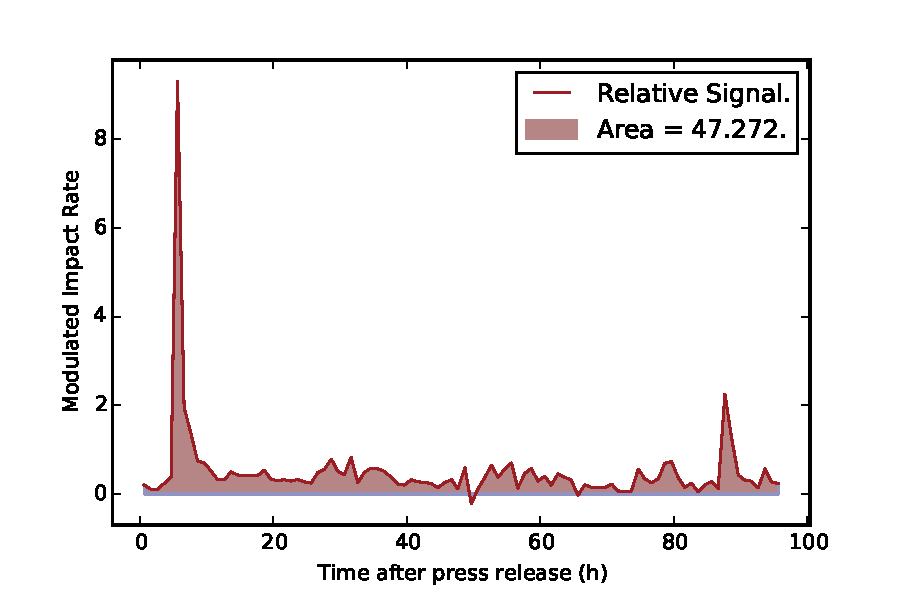
\includegraphics[width=\figwidth]{pics/esa/deep_dreams_modulated_integration.pdf}
	\caption{A measure of the total impact on Twitter by a press release can be obtained by integrating over the difference between a signal corresponding of the average tweet cosine similarity modulated by the relative activity, and a corresponding baseline. This measure does not depend on the typical Twitter activity and so can be used to compare the effectiveness of campaigns of varying size.}
	\label{fig:total_impact_integral_thingy}
\end{figure}
If one wishes to include the number of tweets posted in the impact measure, the result can be computed and visualized nicely by again obtaining a baseline cosine similarity from a period prior to publication and then considering e.g. the cumulative deviation from that following the release, as shown in figure \ref{fig:deep_dreams_cumulative_blabla}.
\begin{figure} %[htb]
	\centering
	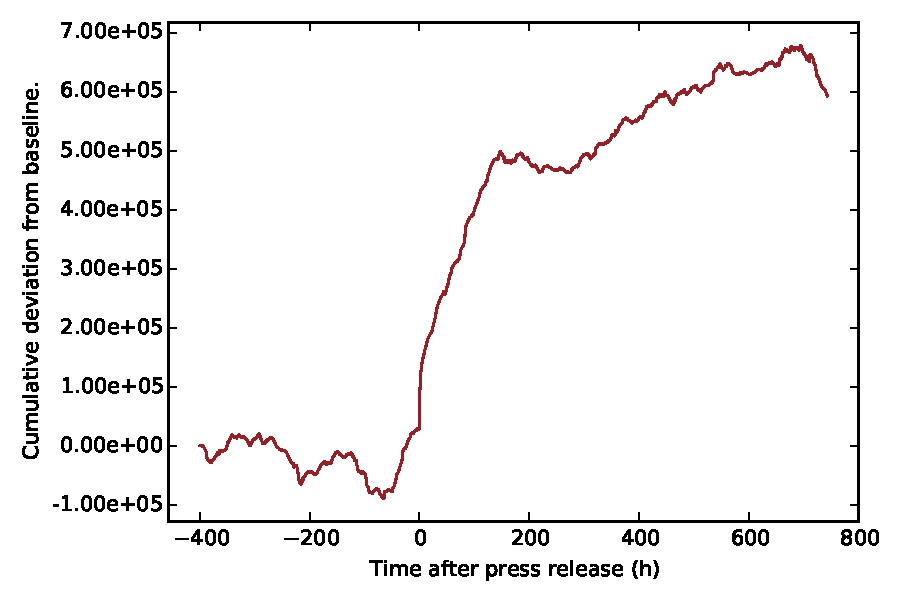
\includegraphics[width=\figwidth]{pics/esa/deep_dreams_tweet_by_tweet.pdf}
	\caption{The cumulative deviation from the mean cosine similarity between the Deep Dreams post and tweets in the period around its release.}
	\label{fig:deep_dreams_cumulative_blabla}
\end{figure}